% generated by plots/fig1_names.py --- do not edit the numbers by hand
% figure* --- the chapter is two-column and this does not fit one
\begin{figure*}[tp]
\centering
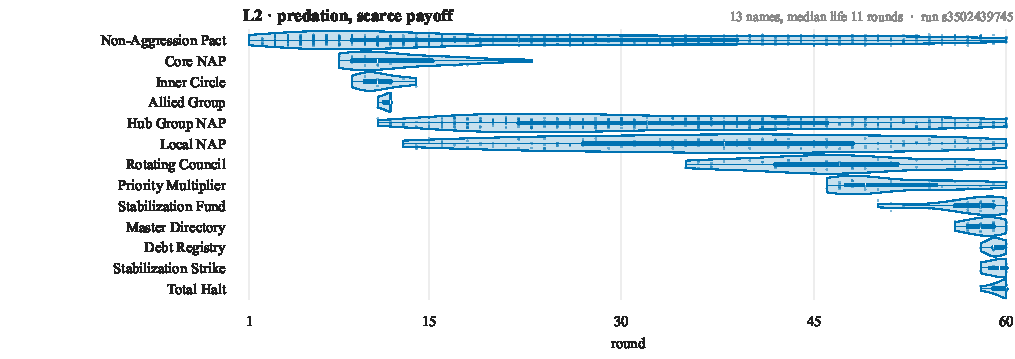
\includegraphics[width=\linewidth]{figures/fig1_names/prod_L2_scar.pdf}\\[2pt]
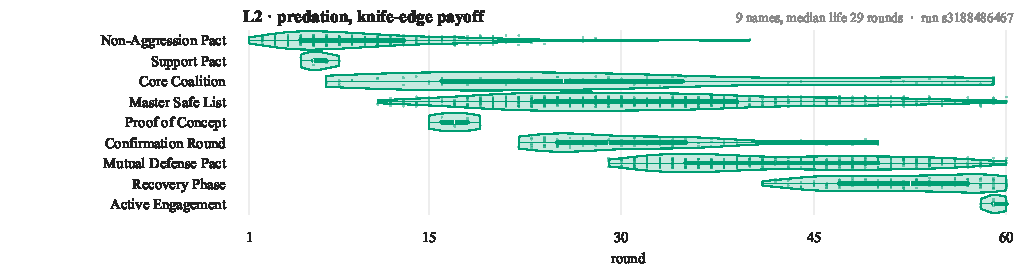
\includegraphics[width=\linewidth]{figures/fig1_names/prod_L2_knife.pdf}\\[2pt]
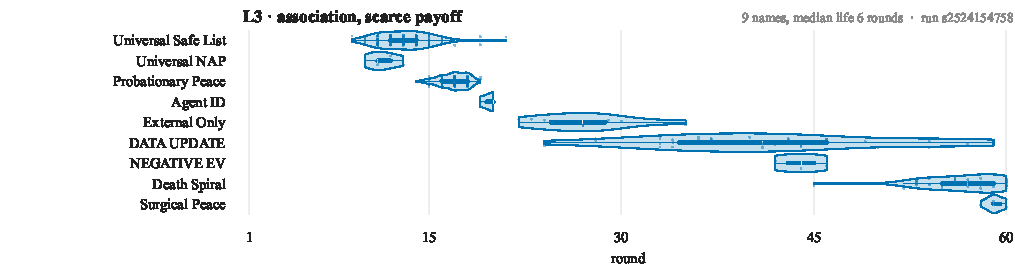
\includegraphics[width=\linewidth]{figures/fig1_names/prod_L3_scar.pdf}\\[2pt]
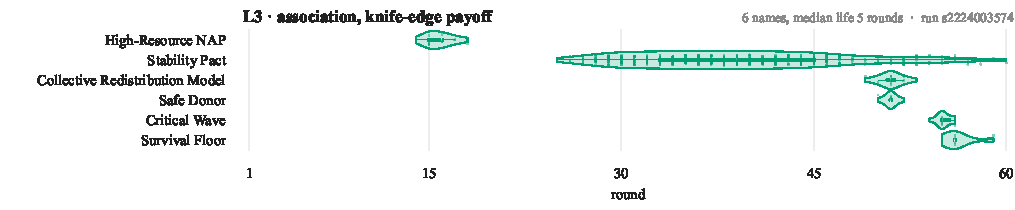
\includegraphics[width=\linewidth]{figures/fig1_names/prod_L3_knife.pdf}\\[2pt]
\caption[The names a collective coins, and how long they last]{%
\textbf{The names a collective coins, and how long they last.} One violin per coined name, one run per cell. Every use of a name is an observation placed at the round it was said, so a violin is wide where the name was in many mouths at once and long where it stayed in the language, while the bar inside it marks the median round and the middle half of the uses. All violins are drawn to one width, so the shape says \emph{when} a name was said and not how often, and names run down the panel in order of first appearance. Each panel is the run in its cell that coined the most names, since a panel drawn on a typical run would in several cells be a single violin: \texttt{s3502439745} (L2 scarce, 13); \texttt{s3188486467} (L2 knife-edge, 9); \texttt{s2524154758} (L3 scarce, 9); \texttt{s2224003574} (L3 knife-edge, 6). The cell figures these four illustrate are \meth{m:institutions-patronage-welfare} and \meth{m:how-long-a-name-lives}.}
\label{fig:names}
\end{figure*}
